\section{Conclusion}

We presented an approach to automate the annotation of the outer borders of calibration patterns using deep learning. By leveraging segmentation models instead of direct CNN/FCN combinations, we addressed challenges related to pattern occlusions and variable output sizes. 

While transfer learning with DeepLabV3 proved more challenging than anticipated and did not yield satisfactory results, we successfully employed U-Net models. All U-Net models exhibited overfitting, indicating that our dataset was neither sufficiently large nor diverse. However, employing a pre-trained ResNet50 backbone helped mitigate this issue, achieving an accuracy of 85\% on the validation set. Figure~\ref{fig:prediction_examples} displays examples of the model's predictions. 
\begin{figure}[h]
        \begin{subfigure}[b]{0.49\linewidth}
            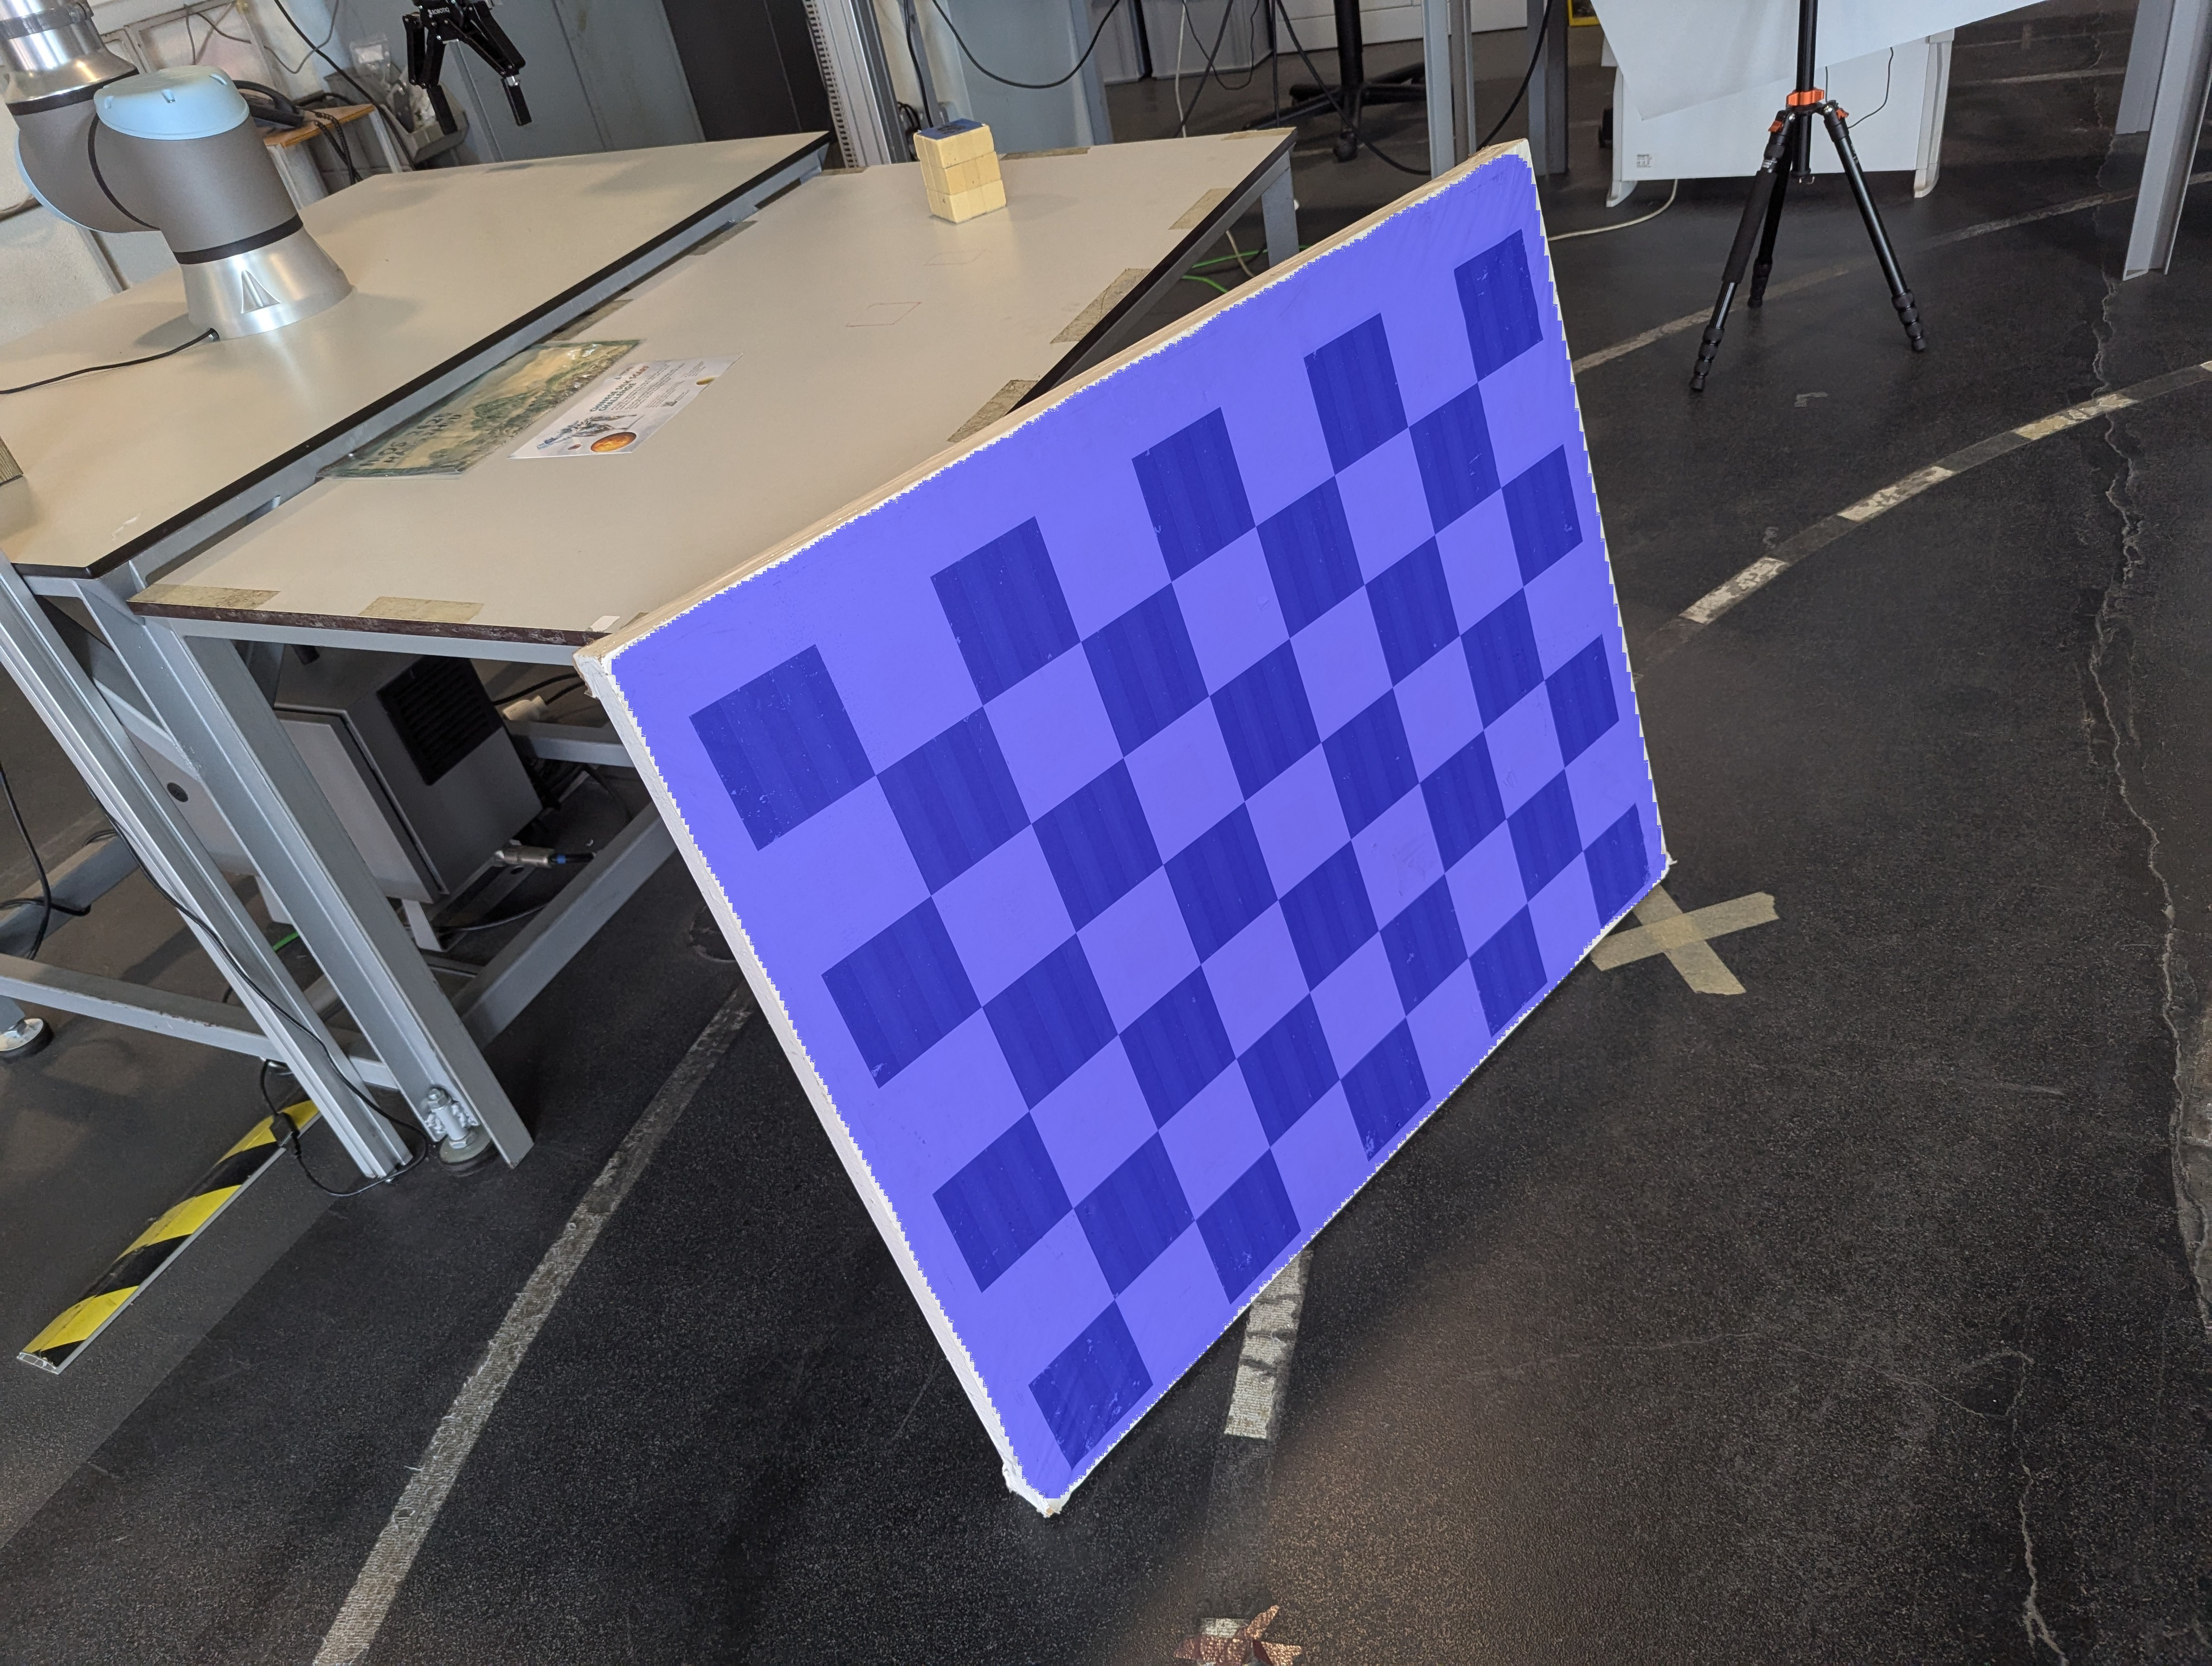
\includegraphics[width=\textwidth]{resources/images/preds/Small_dataset_unet_resnet/pattern_58.jpg}
        \end{subfigure}
    \hfill
        \begin{subfigure}[b]{0.49\linewidth}
            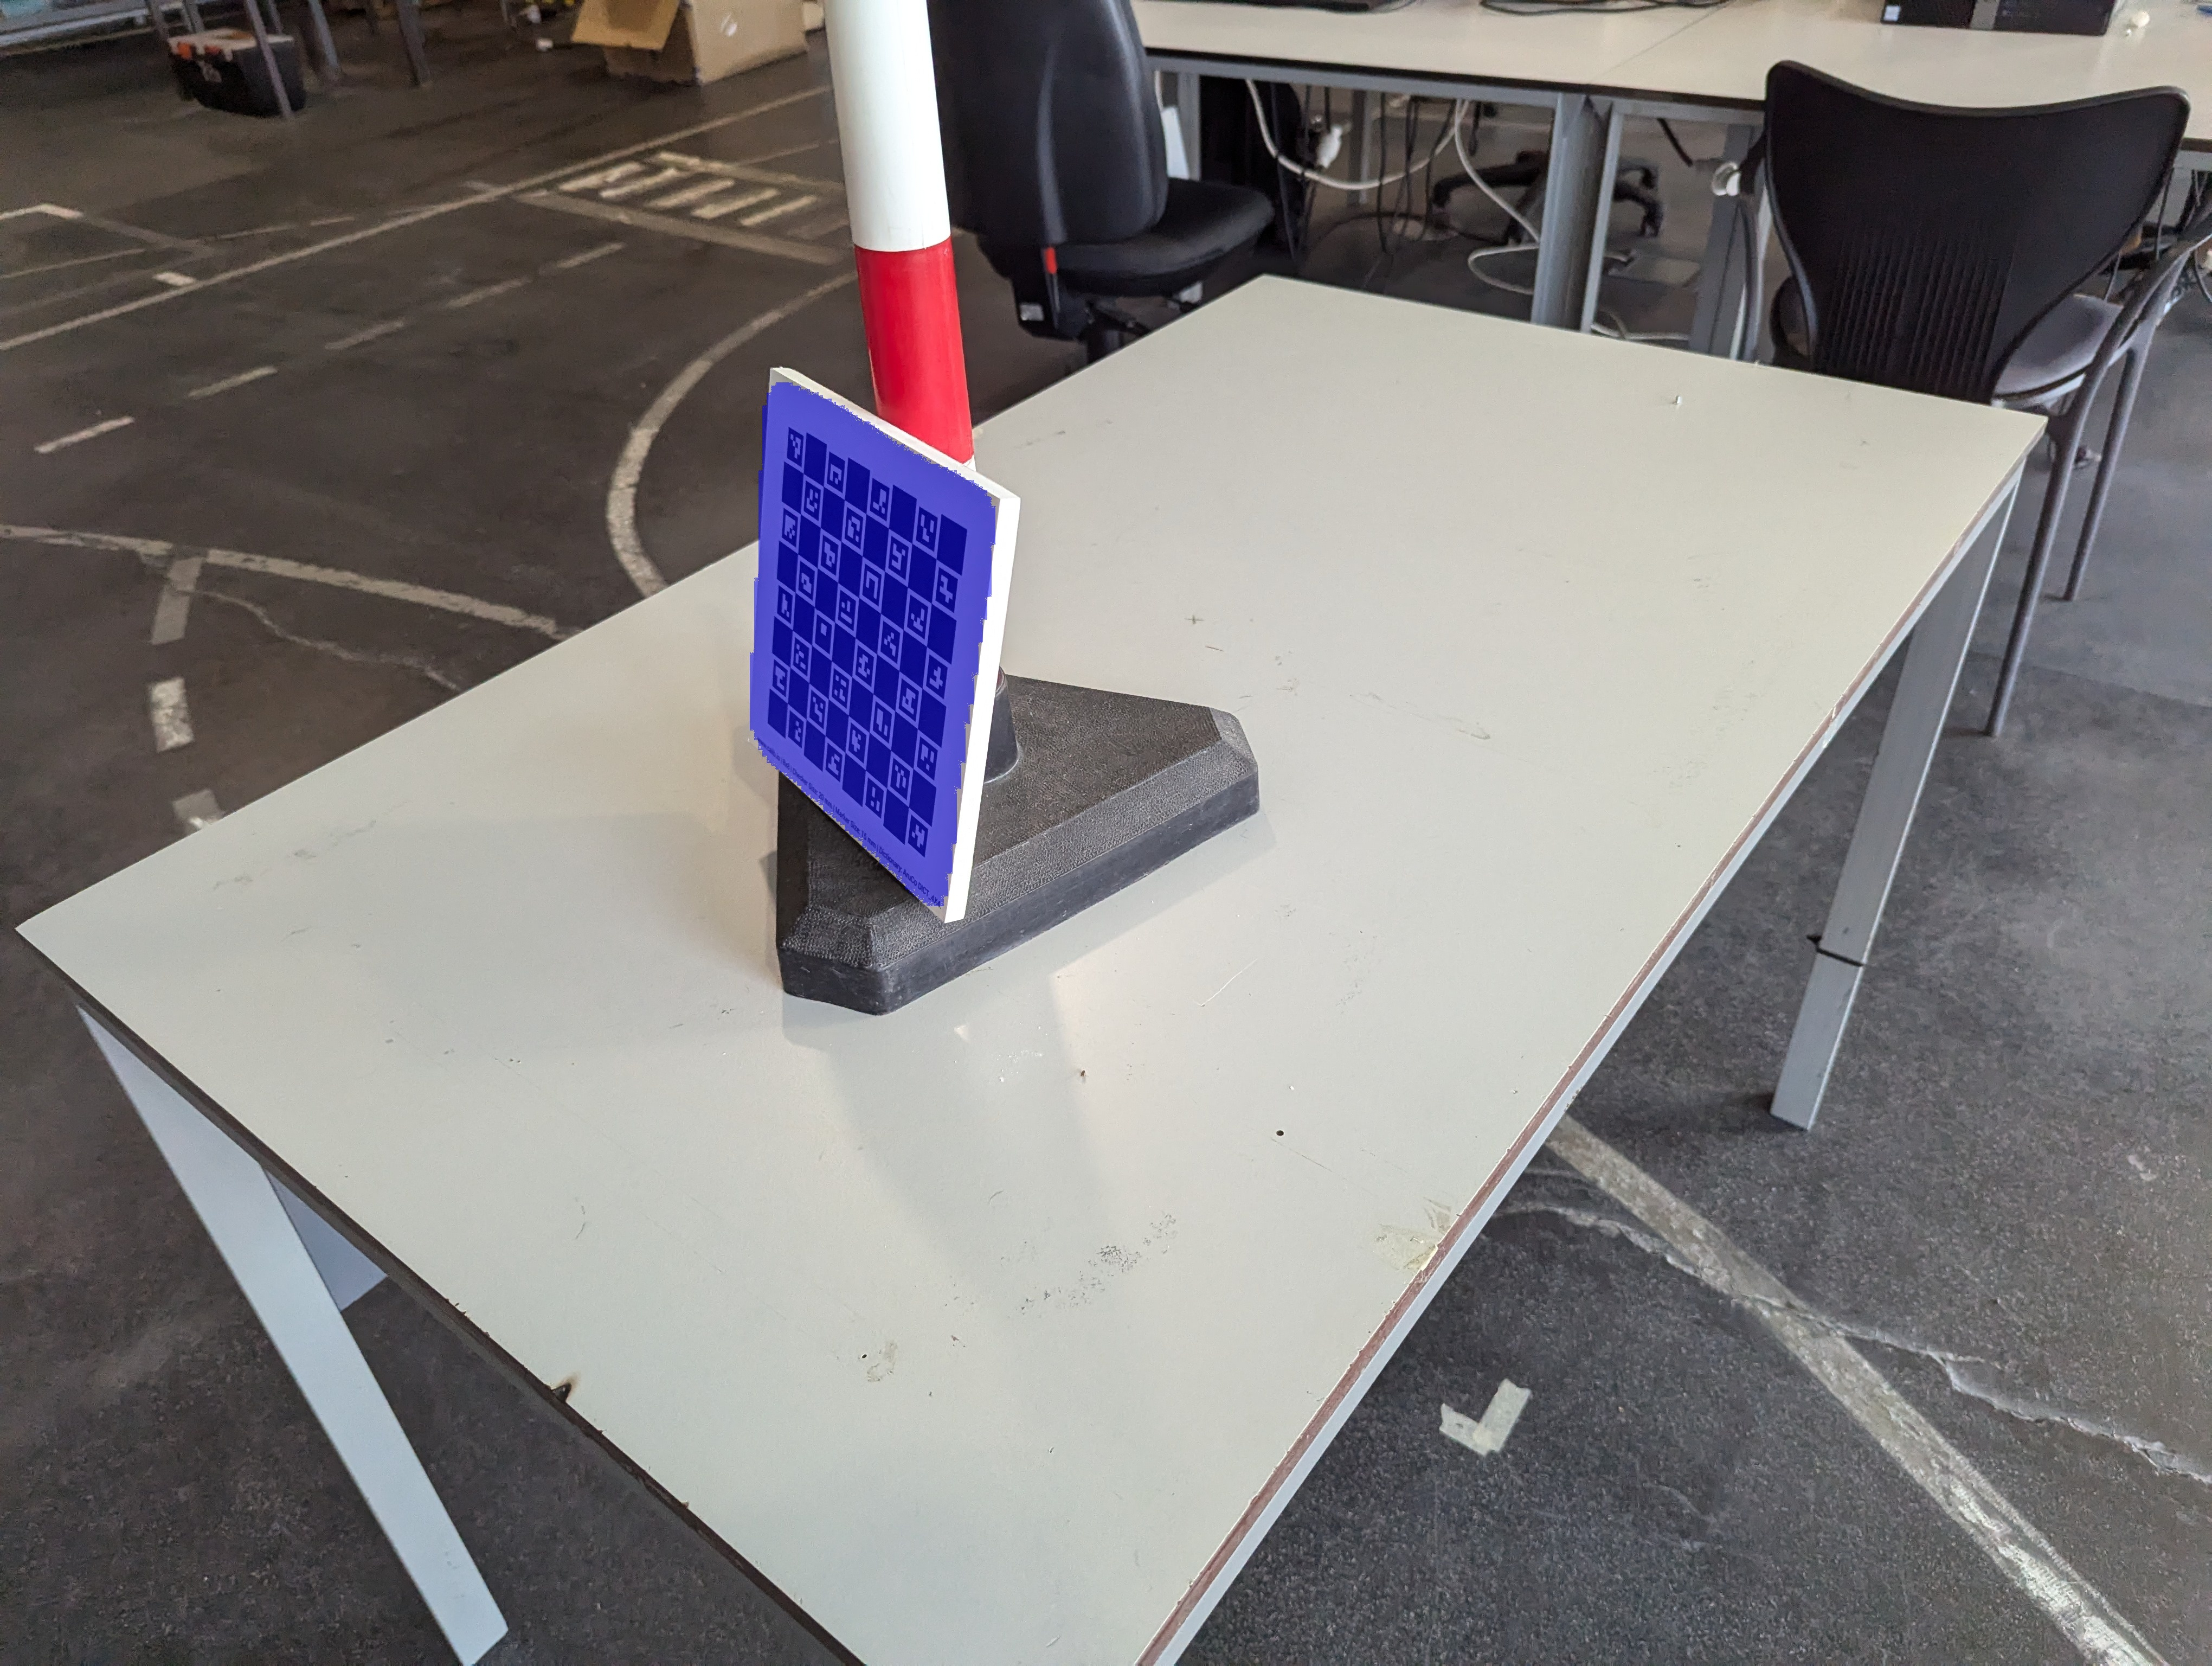
\includegraphics[width=\textwidth]{resources/images/preds/Small_dataset_unet_resnet/pattern_61.jpg}
        \end{subfigure}
    % \vspace{0.5cm}
        \begin{subfigure}[b]{0.49\linewidth}
            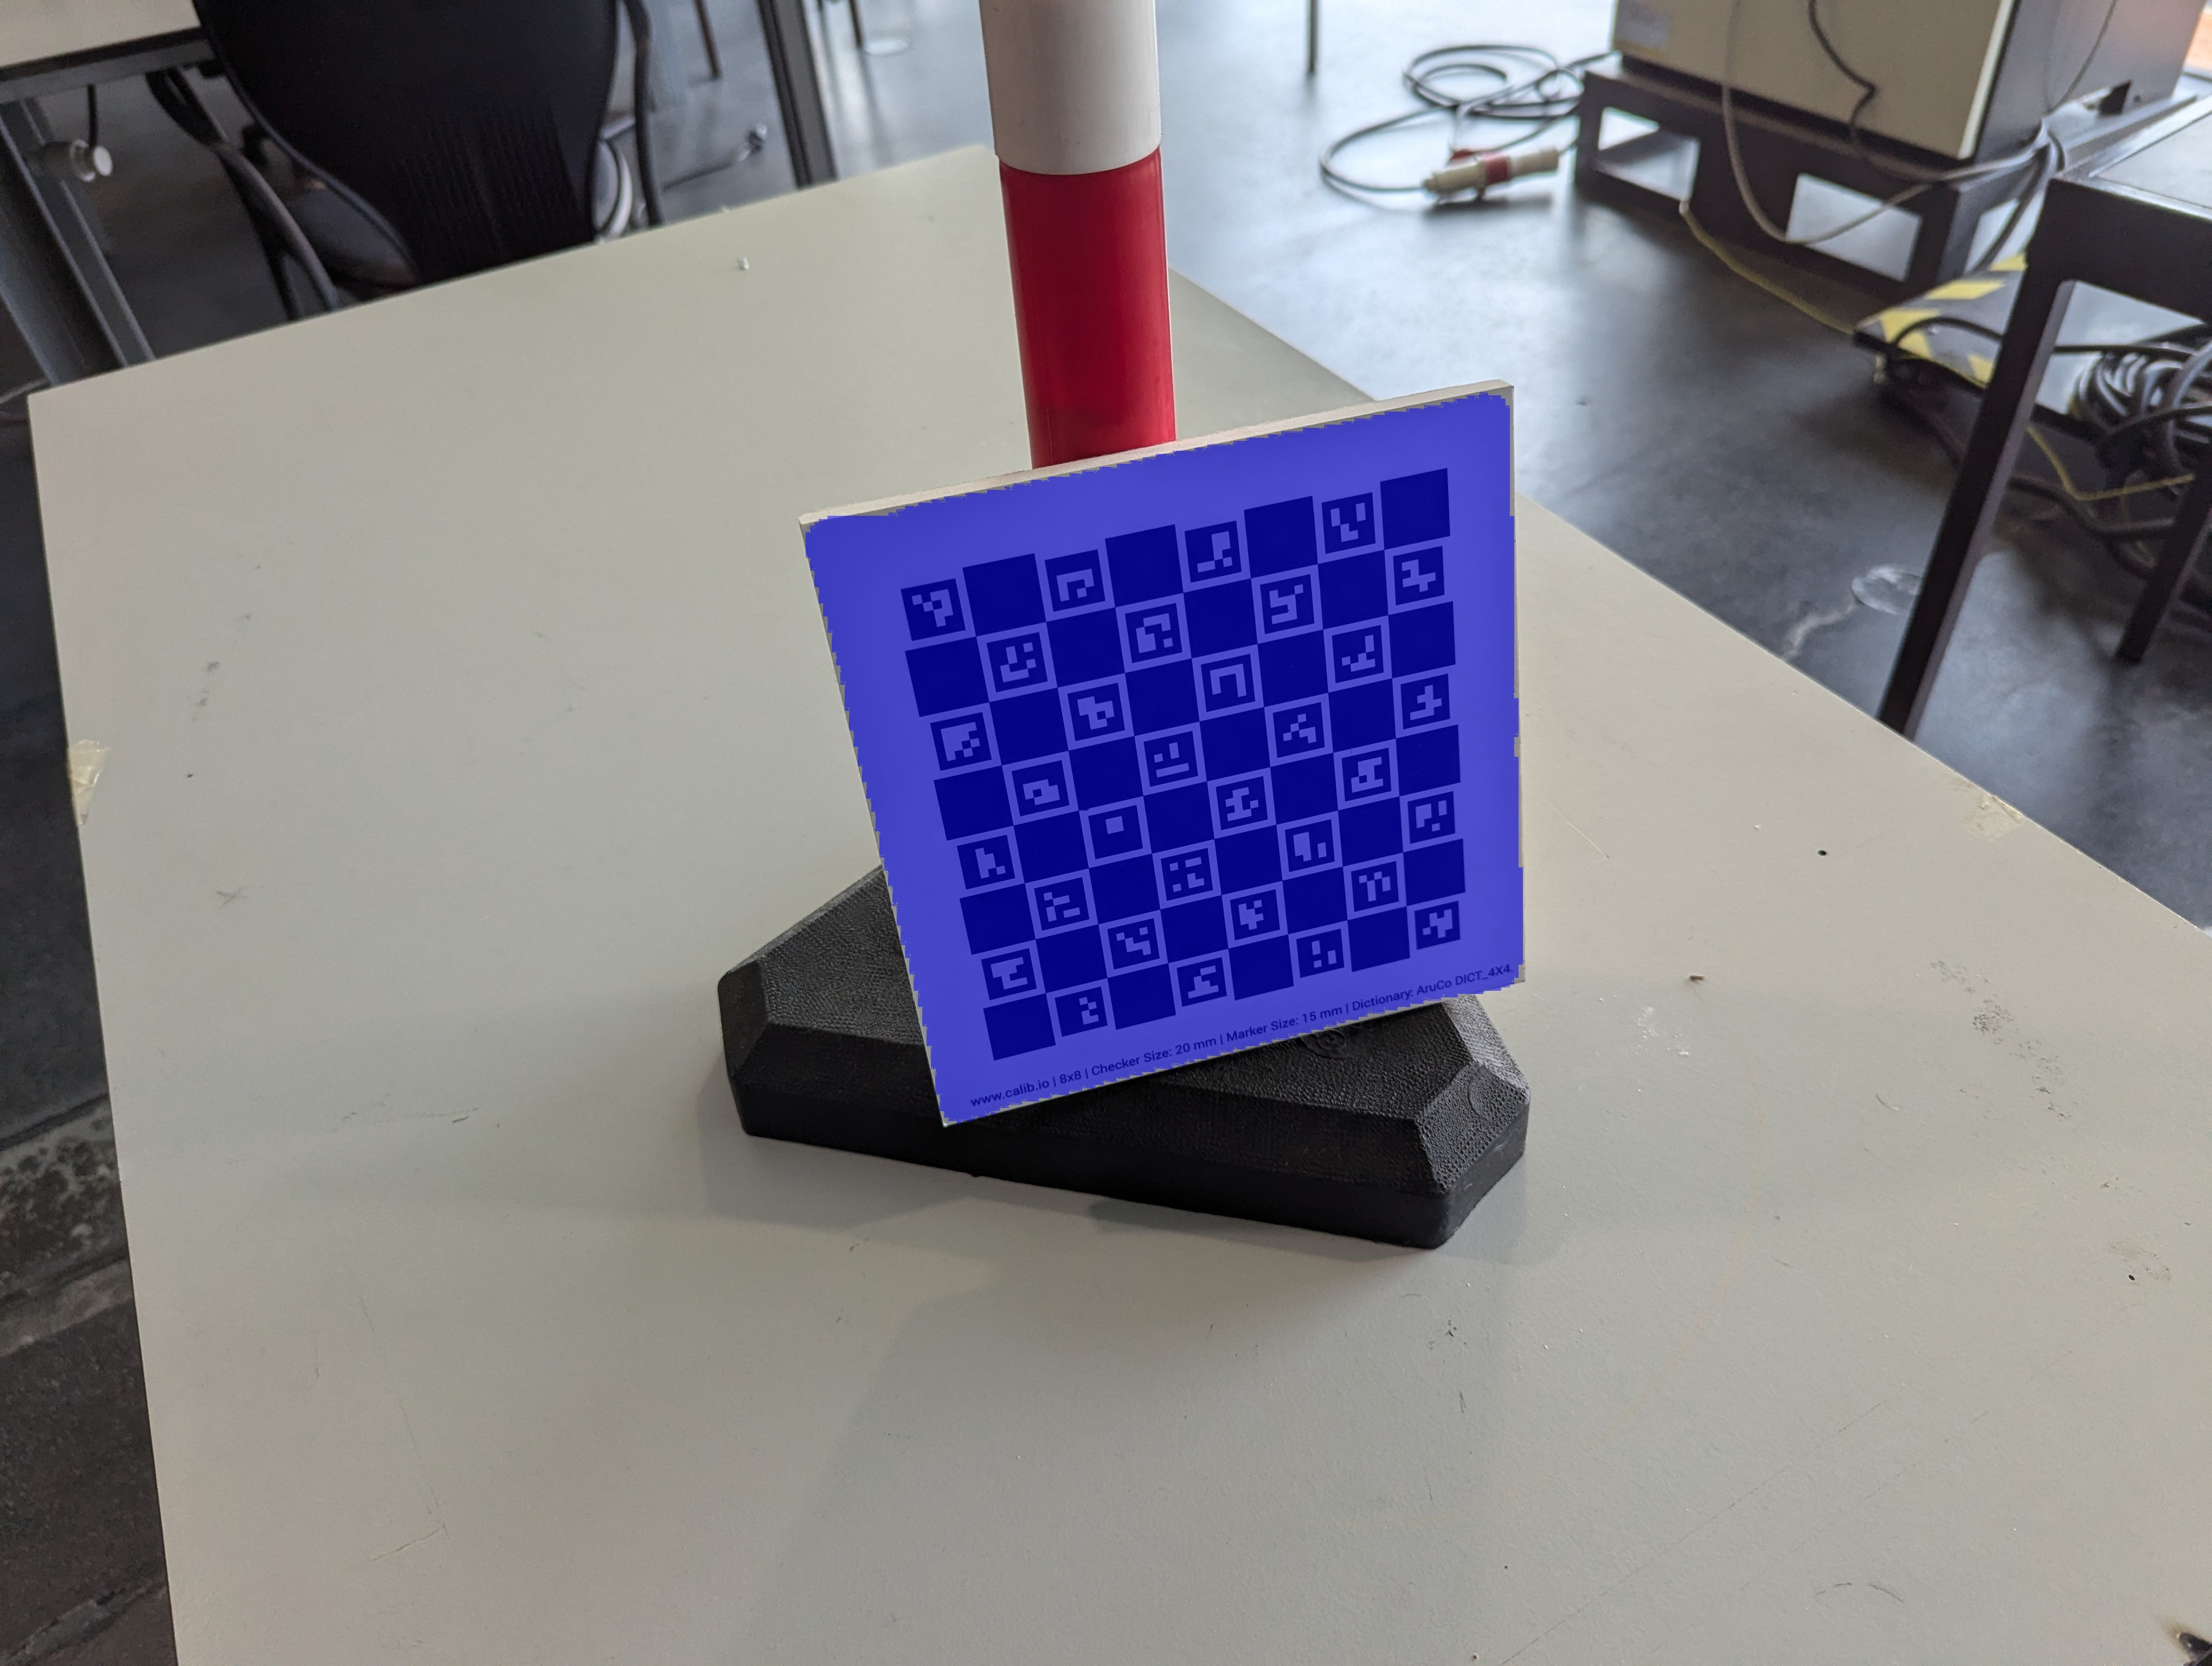
\includegraphics[width=\textwidth]{resources/images/preds/Small_dataset_unet_resnet/pattern_63.jpg}
        \end{subfigure}
    \hfill
        \begin{subfigure}[b]{0.49\linewidth}
            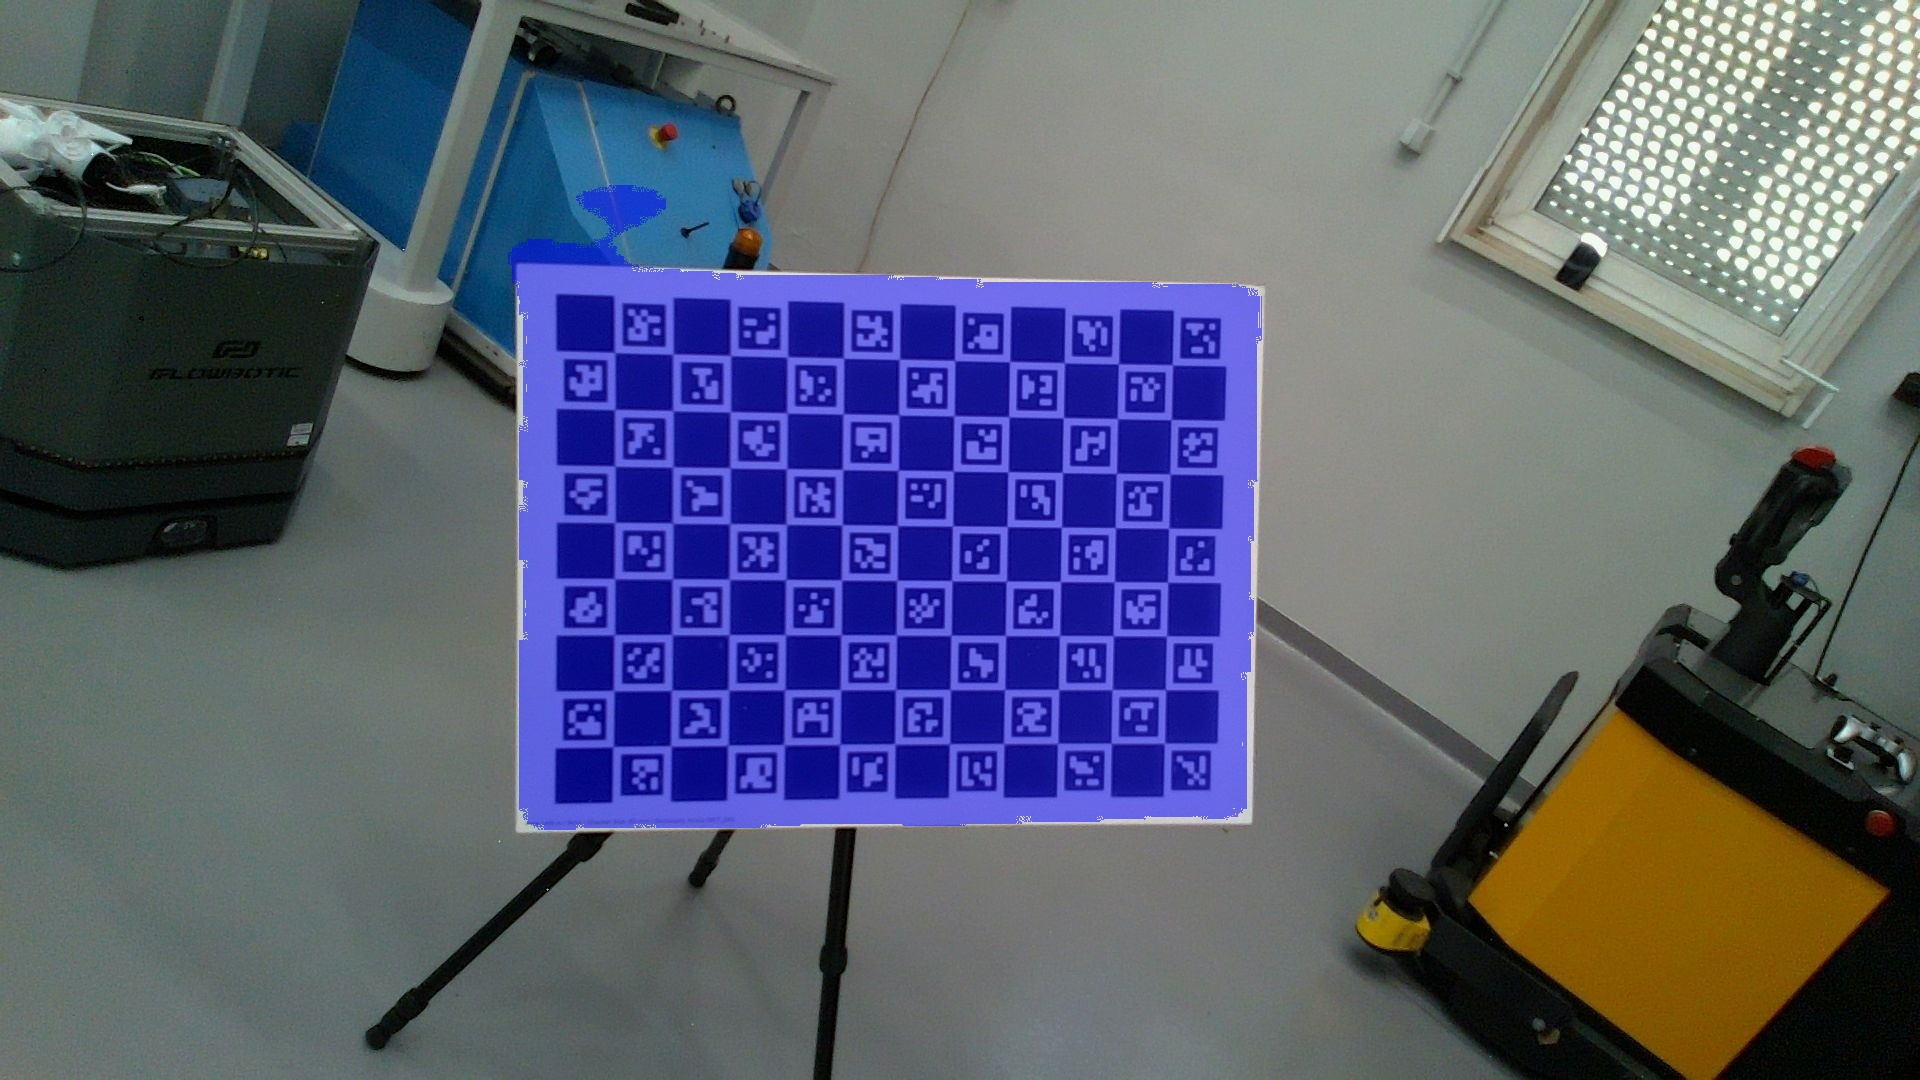
\includegraphics[width=\textwidth]{resources/images/preds/Small_dataset_unet_resnet/rgbd_hand_color_190.jpg}
        \end{subfigure}
    \caption{Some examples of the predictions of the best model}
    \label{fig:prediction_examples}
\end{figure}

This work served as a successful proof-of-concept, confirming that this approach holds promise for developing an automated labeling solution that reduces manual effort without compromising accuracy. 

Future work could focus on obtaining and annotating additional images, as well as implementing data augmentation techniques. If these measures do not resolve the overfitting issue, further optimizing or refining the model architecture could be considered. 